	\documentclass[10pt,a4paper]{report}

% Diff�rentes options pour la classe :
% - taille de la fonte    : 10pt, 11pt, 12pt
% - recto ou recto-verso    : oneside, twoside
% - stade de d�veloppement    : draft, final

% Chargement d'extensions
%\usepackage[latin1]{inputenc}    % Pour utiliser les lettres accentu�es
\usepackage[english]{babel}    % Pour la langue fran�aise

%\usepackage[english,francais]{babel}
\usepackage[latin1]{inputenc}    % Pour utiliser les lettres accentu�es
\usepackage{hyperref}
\hypersetup{
    colorlinks=true,
    linkcolor=black,
    filecolor=black,      
    urlcolor=black,
}
 
\urlstyle{same}
%\usepackage[utf8]{inputenc}
\usepackage[T1]{fontenc}
\usepackage[pdftex]{graphicx}
\usepackage{setspace}
%\usepackage{hyperref}
\usepackage[french]{varioref}
\usepackage{fancyhdr}
\usepackage{color}
\usepackage{colortbl}
\usepackage{amsmath}
\usepackage{float}




\pagestyle{fancy}
\fancyhead[L]{ISTIC}
\fancyhead[C]{}
\fancyhead[R]{\rightmark}


\fancyfoot[L]{Mobile Application Developement}
\fancyfoot[C]{}
\fancyfoot[R]{\textbf{page \thepage}}


% D�but du document
\begin{document}

\begin{titlepage}
%\maketitle



\begin{center}
Tunisian Republic \\
Ministry of Higher Education and Scientific Research

\begin{figure}[!ht]
\centering

\includegraphics [width =3cm]{ucar.png}
\end{figure}

University of Carthage

\vspace{1cm}
\begin{figure}[!ht]
\centering

\includegraphics[width =3cm]{ISTIC.png}
\end{figure}
Higher Institute of Information and Communication Technologies


\vspace*{1cm}


\textbf{\Large{Internship Report}}

\vspace*{0.5cm}
 
\textcolor{black}{\textbf{\Huge{
E-commerce Web and Mobile Application}}}

\vspace*{0.5cm}
\textbf{Host Organization:}\textit{EasyTek}

\begin{figure}[!ht]
\centering

\includegraphics [width =5cm,height=2cm]{easytek2.jpg}
\end{figure}


\vspace*{1cm}

\textbf{\large{Students: \\}}
 \noindent\textbf{Hlel Abdelhedi}
 \noindent\textbf{Ouni Heny }
\vspace*{0.5cm}

Fundamental Bachelor in Computer Sciences 

 
\end{center}





\begin{center}  
\vspace*{1cm}  
College year 2016 - 2017
\end{center}

\end{titlepage}
\newpage
\pagenumbering{roman}
\chapter*{Dedications}
\addcontentsline{toc}{chapter}{Dedications}



We dedicate this work to everyone who has supported and inspired us. Our families. Our parents , our brothers, our sisters . You provide us the end-less support we need to go seize the day. You understand our crazy dreams and you push us forward as we chase them ! Thank you. 
\\*
\\*
To our friends. When life gets tough, you are always there to cheer us up. Thank you for being such amazing friends. I could never do it without you. 
\\*
\\*
To Everyone who we love, Thanks for being so wonderful and kind to us . we appreciate your support and understanding . 
\\*
\\*
Hlel Abdelhedi and Ouni Hani 


\chapter*{Acknowledgment}
\addcontentsline{toc}{chapter}{Acknowledgments}
Before presenting our work,we would like to thank all the people who contributed to the success of our internship and who helped us in the drafting of this report.

\vspace * {1cm}
First of all,We want to express our deep gratitude too ,  to all the EasyTek family especially Mr Lahbib louati for help, relevant explanations and valuable tips that have the greatest impact in the success of the completed project.

\vspace * {1cm}

We would like to thank our internship supervisor, Mr. Mohammed kharat, computer teacher at ISTIC, for his hospitality, the time spent together and the sharing of his expertise on a daily basis.

\vspace * {1cm}
We would also like to thank all our professors  especially Dr Zaineb Trablesi .

\vspace * {1cm}

Finally, our profound gratitude to the Director of the Higher Institute of Information and Communication Technologies Mr. Mongi Besbes  and all members of the administration for the effort and care they given to our successful project.



\tableofcontents    % Table des mati�res
\listoffigures        % Liste des figures
\newpage
\pagenumbering{arabic}
\chapter*{General Introduction}
\addcontentsline{toc}{chapter}{General Introduction}





The major part of news websites have mobile apps aside to them . Since mobile apps are too much portable and easy to use . The push notifications  web services makes building a mobile app  aside to the newspaper website a very suitable solution to make your clients more engaged and loyal to your website . 
 
Hssine bouzara the founder and Director of publication of L'affiche News online news website  has decided to adopt this solution and build own mobile app aside to his website . The mobile demanded application must contain 3 major features: 

\begin{enumerate}
  \item Development of a WordPress plugin which is responsible for sending the push notification if any new post is posted on the website . and retrieve data from the database and and encode  them in JSON format . 
  \item News browsing.
  \item Push notification service integration on the app. 
\end{enumerate}

This project was assigned to me during my summer internship at Mind Engineering .
In the next few pages i will talk with details about the context of my project , the client's need and the design and the developement of the application .

 


	
 


\chapter{Project context}
    %\addcontentsline{toc}{chapter}{}
My project was In the occasion of a summer internship . In the rest of this chapter i will present my host organisation and Then i will explain the main idea and the purpose of my application.  
\section{Company presentation}
\subsection{Company Description}
Mind Engineering is an agency specializing in the design of innovative , efficient and customized software solutions . They are a team of developers, designers and project managers, all experts, passionate about thei	r business and proud of the solutions they offer to their partners.
\subsection{Accomplishements}
Mind engineering had achieved too much success in a very limited period . They have a completed many successful projects since their beginning in 2015 until now  and 
these are some examples : 
\begin{itemize}
\item ISTIC website : 
\begin{figure}[H]
	
\includegraphics[width=10cm]{istic.jpg}
		\caption{\href{http://www.istic.rnu.tn/}{www.istic.rnu.tn} : ISTIC Website}
	\label{istic website}
\end{figure}



\item SOGEFEC (Societe generale froid et climatisation) website : 
\begin{figure}[H]
	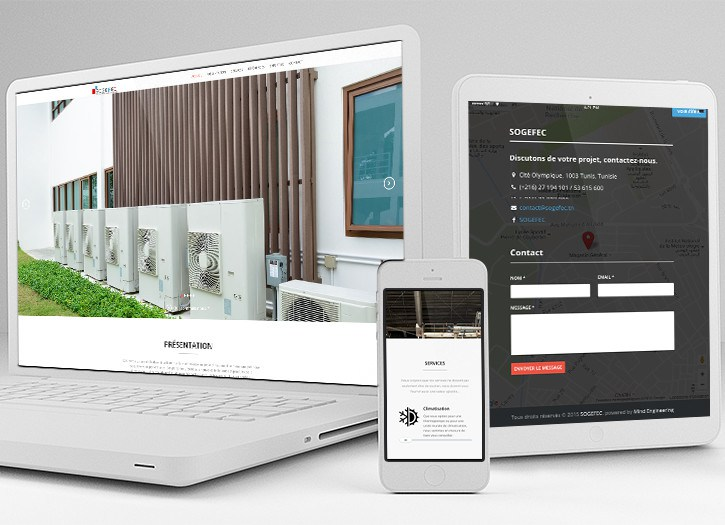
\includegraphics[width=10cm]{sogefec.jpg}
	\caption{\href{http://www.sogefec.tn/}{http://www.sogefec.tn/}  sogefec website}
	\label{istic website}
\end{figure}

\item Jadal online  : 
\begin{figure}[H]
	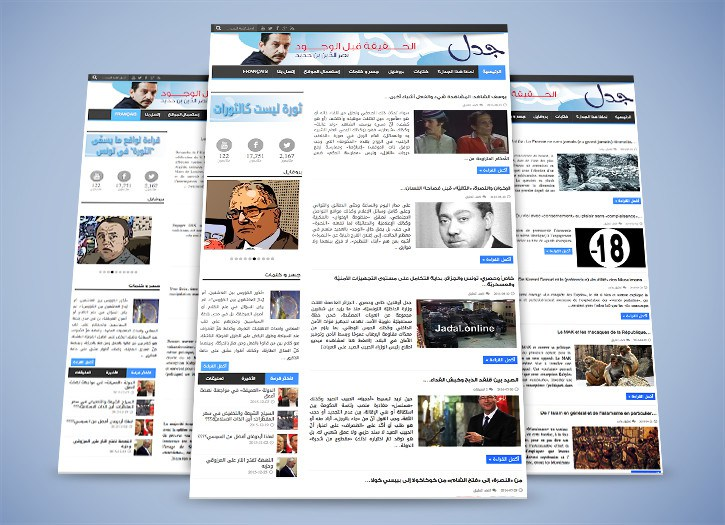
\includegraphics[width=10cm]{jadal.jpg}
	\caption{\href{http://jadal.online/}{http://jadal.online/}  jadal online}
	\label{istic website}
\end{figure}


\end{itemize}


\newpage
\section{Application context}
In this section we will discuss the main purpose of the application . and why every news website should build it's own mobile app . 
\subsection{The noticed rise of mobile devices users and internet users }
The report from the National Telecommunication Forum (INT), published on its website, Tunisians are using a 3G compatible phone, 23.5 percent change their phone every 6 months and 60 percent spend more than 3 hours a day online, against 36 percent between 1 and 3 hours a day and 12 percent within an hour  day.

\subsection{The migration to android }
According to GSM Arena Android will be the most popular mobile OS in the next four years reaching almost 50 percent market share. Meanwhile Windows Phone will catch up and overtake the second place from iOS by 2015 with 20 percent market share.
\subsection{Advantages from using mobile apps for news websites }
Firstly using a mobile app to browse news will create a very good user experience for website followers since mobile apps are very handy and portable which will make the users feel connected and updated with the latest news  . and never forget the simplicity of smartphones using ( it usually takes two or three taps to open the application).
\\*
\\Secondly , Using a mobile app to browse news is economic since you will only require the data and then the application will care for parsing these data , processing them and making show them to the user which will optimize your mobile data using and optimize responding time from the server since we are not requiring extra additional things from the website server like i html , css , javascrit ...etc in websites.
\\*
\\Last but not least , The mobile push notification service is a very useful webservice for news websites  since it offers the possibility for the users to be instantly updated with latest breaking news . 
 \subsection{conclusion}
 To conclude , the current market circumstances and the various advantages of building your news mobile app aside to your apps imposes the necessity of odopting this solution.
 \\Added to that the huge migration to android platforms will make every person think of creating an android app before any other platform .   



\chapter{Requirements Analysis And application design}


\section{Existing Slutions}
In this subsection i will focus on studying some applications which have the same context as my project in order to retain some of  the helpful features proposed by these applications and avoid their drawbacks. 
\subsubsection{CNN NEWS APPLICATION }

\begin{figure}[h!]
	
\includegraphics[width=13cm]{image3.png}
	\caption{Logo OF CNN NEWS }
	\label{cnn logo}
\end{figure}
\begin{enumerate}
  \item Description of the application:
  \begin{description}
  
  \item \underline{Application name:} CNN Breaking US And World News
  \item \underline{Description:}CNN app is   a portal to the latest breaking news  from around the globe   
  \item \underline{App version:}  2.9.4
  \item \underline{Last updated:}  july , 18 , 2016 
  \item \underline{App size:}  40M
  \item \underline{Offered by:} CNN
  \item \underline{Rate:}  4 stars 
   
\end{description}

  \item Criticism of the application :
  
\begin{itemize}
\item Positive points:
\begin{enumerate}
 \item \underline beautiful user interface (material design ) :Material design is a comprehensive guide for visual, motion, and interaction design across platforms and devices . It's is highly recommended to use in android apps since it's is supported by android devices .
 
 	 	
\begin{figure}[H]
 
\includegraphics[width=10cm]{cnn_design.png}
 \caption{CNN UI}
	\label{france24 UI}
\centering
\end{figure}
	


 
 \item Giving the choice to the user to choose wether to receive push notification or not : this step helps to improve the ux (user experience) of the app .
 

\begin{figure}[H]
	
\includegraphics[width=10cm]{cnn_push.png}
	\caption{CNN push notifications}
	\label{CNN push notifications}
\centering
\end{figure}
	

 
 

	

\end{enumerate}  
  
  
 \item Drawbacks: 
 \begin{enumerate}
 \item big size : 40M
  \end{enumerate}  
\end{itemize}  
\item Proposed Solutions And Retained Features :
\\* 
From all the previous features i will retain all the positive ones and i will try to avoid all the drawbacks .  
\\*
so to summarize the product must present these features:  
\begin{itemize}
\item beautiful material  design  
\item speed and performing application 
\item light weight app 
\item giving the user the choice whether to receive push notifications or not
\end{itemize}


\end{enumerate}
 \newpage
 \subsubsection{FRANCE 24}
\begin{figure}[h!]
	
\includegraphics[width=7cm]{france24.png}
	\caption{Logo of France 24  }
	\label{france24}
\end{figure}
	
\begin{enumerate}
  \item Description of the application:
  \begin{description}
  
  \item \underline{Application name:} France 24 
  \item \underline{Description:} France 24 mobile app is an application which will keep up to date with international news .   
  \item \underline{App version:} varies with device 
  \item \underline{Last updated:} August 9, 2016  
  \item \underline{App size:}  varies with device but big anyway 
  \item \underline{Offered by:} France Médias Monde
  \item \underline{Rate:}  4.2 stars 
   
\end{description}

  \item Criticism of the application :
  
\begin{itemize}
\item Positive points:
\begin{enumerate}
 \item \underline Breaking news popups when the app is in foreground . 


 	
\begin{figure}[H]
 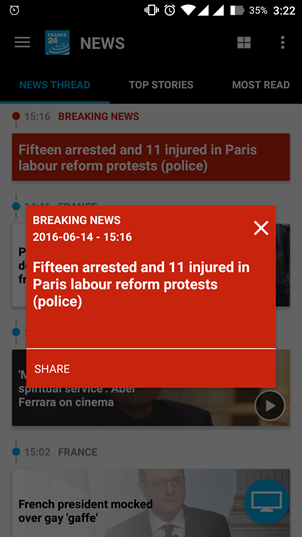
\includegraphics[width=10cm]{france24_popup.png}\caption{France popup}
	\label{france24 poopup}
\centering
\end{figure}
 
 
 \item \underline Push notifications : 
 \\*
 \\*
   \begin{figure}[H]

\includegraphics[width=10cm]{france24_push.png}\caption{France push notifications }
	\label{france24 notifications}
\centering
\end{figure}
 

  \item \underline Beautiful UI .

  
  \begin{figure}[H]
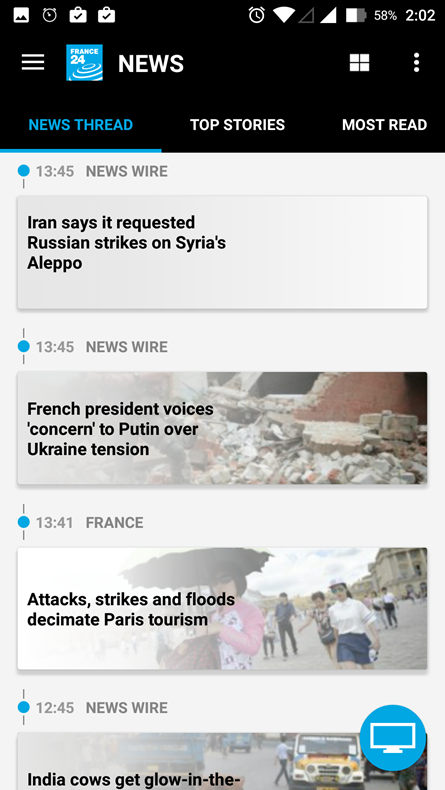
\includegraphics[width=10cm]{france24_ui.png}
\caption{France 24 UI }
	\label{france24 ui}
\centering
\end{figure}
 
\end{enumerate}  
  
  
 \item Drawbacks: 
 \begin{enumerate}
 \item big size 
  \end{enumerate}  
\end{itemize}  
\item Proposed Solutions And Retained Features :
\\* 
From all the previous features i will retain one feature which is the manner how the posts are designed to show with a little modification .


\end{enumerate}
 \newpage
 
 \subsubsection{ASSABAH NEWS : }


\begin{figure}[H]
	
\includegraphics[width=7cm]{assbah.jpg}
	\caption{Logo of assabah news }
	\label{imag3}
\end{figure}
\begin{enumerate}
  \item Description of the application:
  \begin{description}
  
  \item \underline{Application name:} Assabah News 
  \item \underline{App version:} 1.0
  \item \underline{Last updated:} October 10, 2014
  \item \underline{App size:}  :  2.9M
  \item \underline{Offered by:} Orange tunisie 
  \item \underline{Rate:}  4.2 stars 
   
\end{description}

  \item Criticism of the application :
  
\begin{itemize}
\item Positive points:
\\* 

light weight app
 
  
  
 \item Drawbacks: 
\\the ui is not very beautiful

\begin{figure}[H]
	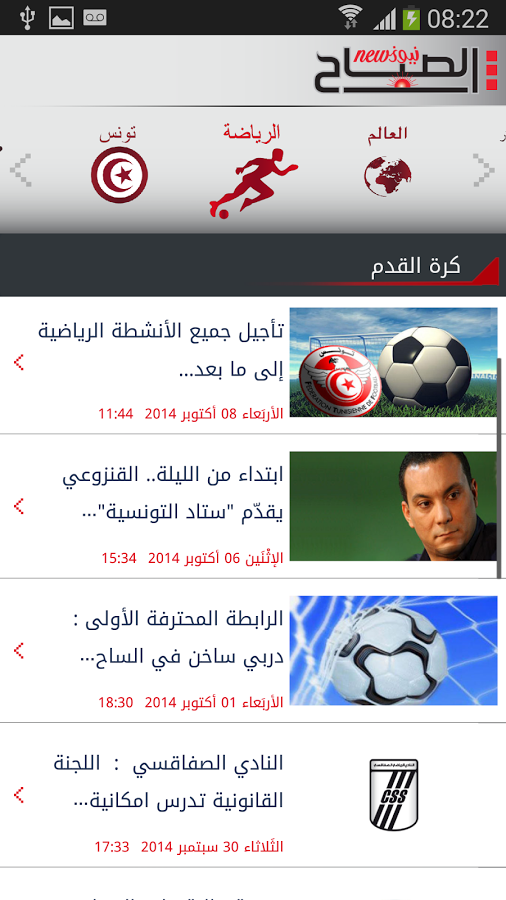
\includegraphics[width=7cm]{assabah_news.png}
	\caption{Assabah news UI }
	\centering
	\label{imag3}
\end{figure}
  
\end{itemize}  
\item Proposed Solutions And Reatained Features :
\\* 
From all the previous features i have been impressed by the little size of the application that's why i will try to make it lightweight as possible .

\end{enumerate}

\section{Requirements Analysis}


\subsection{Informal Requirements Analysis}

\subsubsection{Functional Requirements Analysis}

\begin{itemize}
\item Functionalities:

\begin{itemize}
\item browse news divided by main categories : politique ,  economie , ... (vertical navbar ) , and small categories : ce que je pense ,  (horizontal navbar) .
\item Integrate push notifications service in the app and in the website by developing a WordPress  plugin (php code ) 
\end{itemize}

\item Project Dependencies  : 
\begin{itemize}
\item 	The application must communicate with the website database by using the plugin which must be installed on the WordPress website .
\item The push notification service must communicate with  google servers since we are using the google cloud messaging (GCM)  for push notifications . And then the servers responds with a registration id  which will be sent to the plugin which will insert it in the website?s database to use it later when sending the push notifications  
\end{itemize}

\end{itemize}

\subsubsection{Non Functional Requirements}


\begin{itemize}
\item 	Code must be clear and  commented for future evolutions . 
\item 	Ergonomics : the application must  have a friendly and easy to use UI.
\item  Security : the application must respect the confidentiality of data .
\item 	Ensure the integrity and consistency of data in each update, and each insertion .
\item 	Portability : the plugin must work with every WordPress website , and the app must be generic as much as possible 
 
\end{itemize}

\subsection{Semi-formal Requirements Specification }


\begin{itemize}
\item use case diagrams :

\begin{itemize}
\item browse news :
\begin{figure}[h!]
	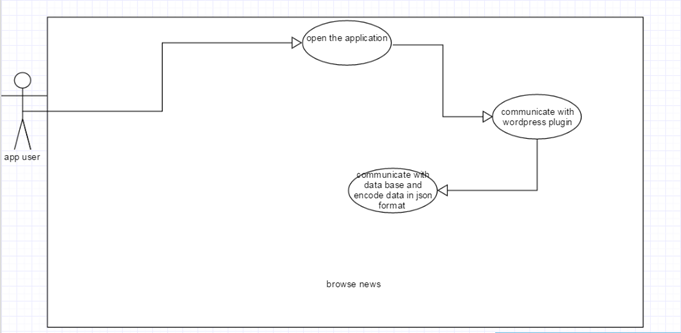
\includegraphics[width=13cm]{usecase1.png}
	\caption{Browsing news use case}
	\label{imag3}
\end{figure}
\item push notification :
 \begin{figure}[h!]
	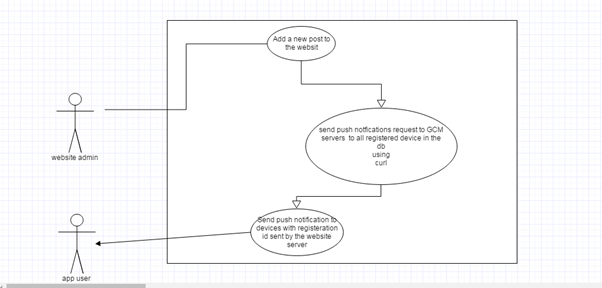
\includegraphics[width=13cm]{usecase3.png}
	\caption{Push notification use case diagrams}
	\label{imag3}
\end{figure}
\end{itemize}
\item	Presentation of actors :
\begin{itemize}
\item App user : the user of the app 
\item Website admin : the person or the group of persons who are responsible for updating the database or postings new news on the website .

\item  Browse news : the actor opens the app the app will send AJAX request to the plugin . The purpose of these requests is asking for receiving data using json format . then the wordpress plugin which is already connected to the database selects the suitable data using the category name to select it right and then it encodes the data retrieved and responds the ajax call with the required data in JSON format .
\item Push notification : the website admin adds a new post on the site invokes the sending of curl request to GCM servers for each device registered on the site . and finally the GCM servers sends push notifications to these devices or updates the app if it?s in foreground .
\end{itemize}

\end{itemize}

\subsection{Application design}
\subsubsection{Sequence diagrams}
\begin{itemize}
\item \textbf{Data extraction sequence diagram:}
 	 	
\begin{figure}[H]
 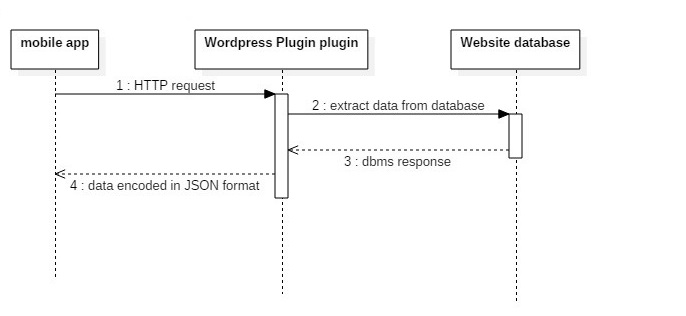
\includegraphics[width=10cm]{sequence2.jpg}
 \caption{Data extraction sequence diagram}
	\label{Data extraction sequence diagram}
\centering
\end{figure}
	
\item \textbf{plugin sequence diagram:}
\begin{figure}[H]
 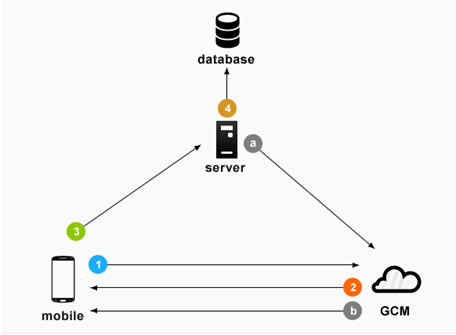
\includegraphics[width=10cm]{sequence1.png}
 \caption{Data extraction sequence diagram}
	\label{Data extraction sequence diagram}
\centering
\end{figure}
\item \textbf{Push notification squence diagram:}

\begin{itemize}
\item Push notification squence diagram : 
 \begin{figure}[h!]
	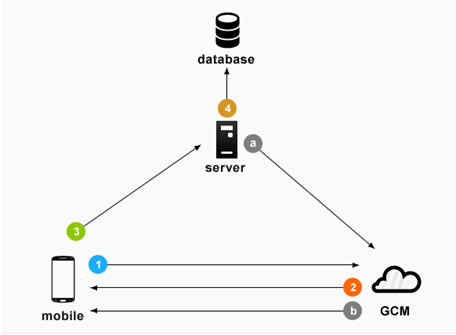
\includegraphics[width=13cm]{sequence1.png}
	\caption{Push notifications sequence diagram}
	\end{figure}
\item Description :
\\*  
\\1. First android device sends sender id, application id to GCM server for registration. 
\\*
\\2. Upon successful registration GCM server issues registration id to android device. 
\\*
\\3. After receiving registration id. device will send registration id to our server 
\\*
\\4. Our server will store registration id in the database for later usage 
\\*
\\(a) Whenever push notification is needed, our server sends a message to GCM server along with device registration Id (which is stored earlier in the database)
\\*
\\(b) GCM server will delayers that message to respected mobile device using device registration id 
\end{itemize}
\end{itemize}

\subsubsection{UI Design}
 To have an idea ,about how the UI of the app will be , i have deisgned some interfaces using adobe photoshop :
 \begin{itemize}
 \item Home Screen
 

 
\begin{figure}[H]
\centering
 
\includegraphics[width=6cm]{home_screen.jpg}
 \caption{Home screen UI}
 
	\label{home screen ui}

\end{figure}
\item Slide out menu :
 \begin{figure}[H]
\centering
 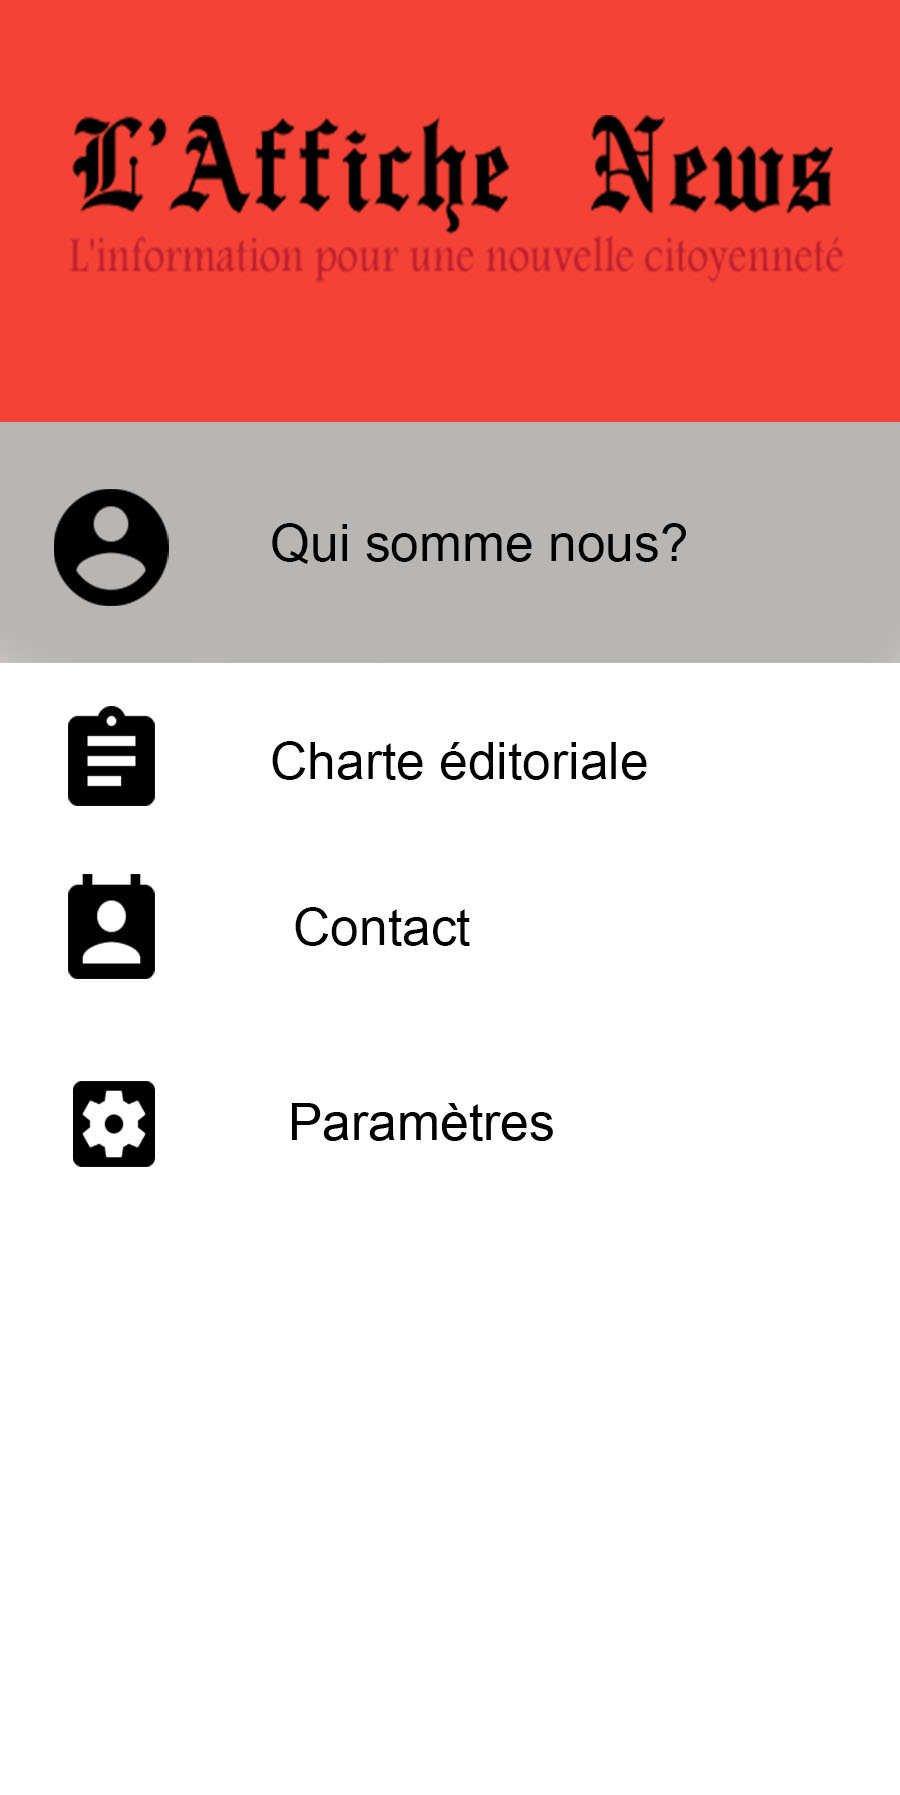
\includegraphics[width=6cm]{slide_out.jpg}
 \caption{Slide Out menu}
 
	\label{slide out menu}

\end{figure}
 \end{itemize}

\textbf{Note:} You may notice some differences between these interfaces and the actual application design because of updates and new ideas during the developement

\chapter{Development}

\section{Development environment}
\subsection{hardware environment :}
To develop the project i used un smartphone android lenovo k3 note ( processor : mtk 1.8ghz , 2gb of ram , 5.5 screen ... ) and a laptop  DELL inspiron 15 : 
\begin{itemize}
\item Intel (R) Core i3-3217 CPU
\item 4GB RAM
\item 500GB Hard Disk
\item 15 inch lcd screen
\end{itemize}
\subsection{Software environment: }
\begin{itemize}
\item	windows 7 Edition Integrale 64bits
\item	MySQL as a DBMS 
\item	Intel XDK (developement kit ) 
\item	Atom and Brackets as IDE
\item 	android 6.0
\item 	Adobe photoshop cs6
\item 	WordPress 
\end{itemize}
\section{Choice of development tools}
\begin{itemize}
\item \textbf{DBMS:MySQL} is the dbms already used by L'affiche news website
\item \textbf{Editors:Brackets and Atom } Two open source IDEs characterized  by the massive number of plugins available for these two editors.
\item \textbf{IntelXDK:} is a development kit created by Intel to create native apps for mobile phones and tablets using web technologies like HTML5, CSS and JavaScript. Apps are compiled online via the Cordova platform for making cross-platform apps . i have choose this platform since the required application is Hybrid application 
\\*
\\*
This app is developed using Hybrid mobile apps because it will accelerate the developement and facilitate the developement for the mobile app developer . It will also make the app easy to adapt to ios based smart phones.

\end{itemize}

\chapter{Internship Achievements}

The application is fully developed and  now available at Google Play Store in 1.0.2 version .
\\*
\\* 
The application's name is : "l'Affiche News TN" . It's size is 3.5 M , it's number of installations is between 10 and 50 And it is 5 stars rated by it's all users .
\\*
\\*
\begin{figure}[H]
	
\includegraphics[width=13cm]{play.png}
	\caption{L'affiche news at playstore}
	\label{play}
\centering
\end{figure}
The website URL is : \url{http://laffichenews.tn/}

These are some screen shot taken from the main parts of the application :

\begin{figure}[H]
\centering
	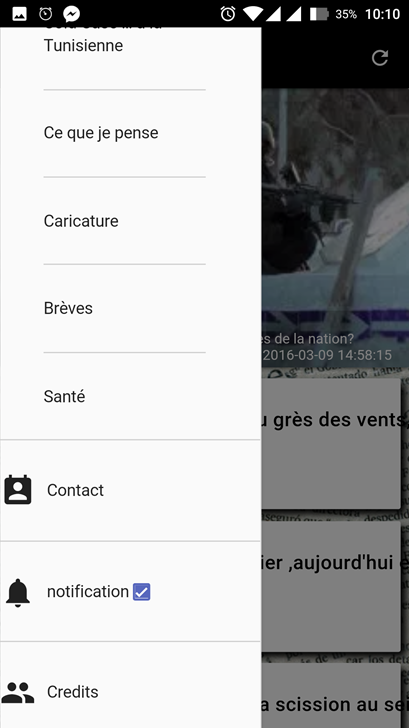
\includegraphics[width=8cm]{screenshot1.png}
	\caption{Slide out menu}
	\label{screenshot}

\end{figure}

\begin{figure}[H]
\centering
	
\includegraphics[width=8cm]{screenshot2.png}
	\caption{Home screen}
	\label{screenshot}

\end{figure}

\begin{figure}[H]
\centering
	
\includegraphics[width=8cm]{screenshot3.png}
	\caption{Subcategorie}
	\label{screenshot}

\end{figure}

\begin{figure}[H]
\centering
	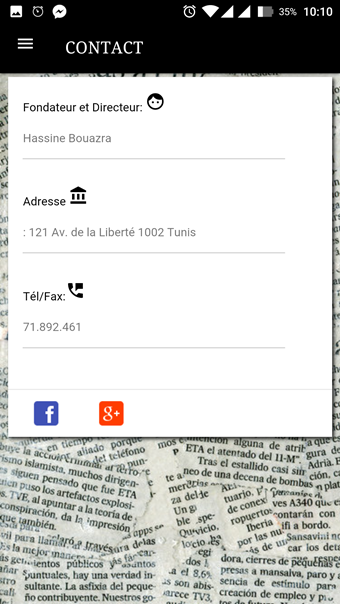
\includegraphics[width=8cm]{screenshot4.png}
	\caption{Contact page}
	\label{screenshot}

\end{figure}


\begin{figure}[H]
\centering
	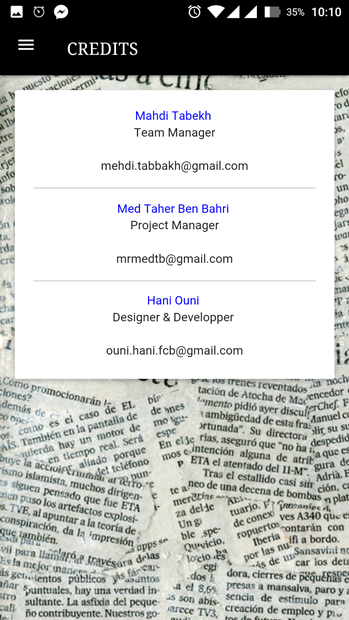
\includegraphics[width=8cm]{screenshot5.png}
	\caption{Credits page}
	\label{screenshot}

\end{figure}

\begin{figure}[H]
	\centering
	
\includegraphics[width=8cm]{screenshot6.png}
	\caption{Reading article page}
	\label{screenshot}

\end{figure}


\chapter*{General conclusion et Perspectives}

For me it was a very nice and wonderful experience to pass my summer internship with the Mind engineering family . It was such an Honor to know these person i have learned a lot of things . 
\\I learned new things such as how to code with php , how to use  AJAX , How to develop a site with wordpress 
.
\\ 
\\ I learned extend also my previous skills and took the to a new level such as jquery , css , javascript , UI frameworks  and mobile developement life cycle .
\\*
But what really made this internship spectacular is to pass a whole 2 months with these people and , learn from their experiences  and to be professional , Timely , And exact like they are .
\\*
\\*
In the future I can see my application more optimized and more performing . And perhaps built for IOS platforms.
\bibliographystyle{plain}
\bibliography{biblio.bib}



% Fin du document
\end{document}

%hhhhhh 